\documentclass[a4paper,11pt]{report}
\usepackage[utf8]{inputenc} 
\usepackage[romanian]{babel}
\usepackage{url}
\usepackage{a4wide}
\usepackage[bookmarks, bookmarksopen=true, bookmarksnumbered=true]{hyperref}
\usepackage{graphicx}
\linespread{1.3}
\addtolength{\parskip}{0.6\baselineskip}

\renewcommand{\title}{OpenCad.org}
\newcommand{\subtitle}{Proiectarea unei aplicaţii CAD pentru arhitectură}
\renewcommand{\author}{Silviu-Georgian Aprozeanu}
\newcommand{\teacher}{prof. dr. ing. Florica Moldoveanu}

\newcommand{\col}[1]{@{\hspace{0.01\textwidth}}p{#1\textwidth}@{\hspace{0.01\textwidth}}}

\newtheorem{definition}{Definiţia}[chapter] 
\newtheorem{statement}{Propoziţia}[chapter]

\begin{document}
	\begin{titlepage}
\null \vfill
	\begin{center}
{\Huge \title{}}
	
{\Large \subtitle{}}
	\end{center}
\vfill
	\begin{flushright}
		\begin{tabular}{ll}
Absolvent & \author{} \\
Profesor îndrumător & \teacher{}
		\end{tabular}
	\end{flushright}
\vskip 2cm
	\begin{center}
\small Bucureşti, \today
	\end{center}
	\end{titlepage}
	\pagenumbering{roman}
	\begin{abstract}
    Prezentare a proiectului OpenCad.org cît şi a tehnologiilor folosite în 
elaborarea lui, a scopurilor acestui proiect, a modului în care a fost
organizată construcţia sa, detalii de implementare şi o privire obiectivă a
obiectivelor îndeplinite şi a planurilor de viitor.

    \end{abstract}
\tableofcontents \listoftables \listoffigures \clearpage
	\pagenumbering{arabic}
	\pagestyle{headings}
	\chapter{Introducere}

OpenCad.org este un proiect iniţiat de autor în anul 2005 cu gîndul de a deveni 
o unealtă de real folos în activitatea de proiectare în domeniul arhitecturii.

Pornit de la o pasiune personală pentru domeniu, ideea acestui proiect vine ca 
o reacţie a curentului open-source, în care din ce în ce mai mulţi programatori 
vor să încerce să ofere soluţii performante şi în acelaşi timp gratuite. Deşi 
această primă determinare a proiectului nu a fost hotărîtoare, desigur eternele 
aventuri în lumea proiectării 3D ale vieţii pre-universitare au avut un rol 
decisiv în hotărîrea temei pentru acest proiect de diplomă.

Proiectul nostru are un slogan, care traducerea în engleză a sintagmei 
``Construieşte, nu desena". El reprezintă tema acestui proiect, anume izolarea 
activităţii creative de proiectarea a spaţiilor de locuit sau a clădirilor cu 
diverse scopuri de activităţile de desenare, de cunoştinţele stricte de desen 
tehnic, de teoria proiecţiilor tridimensionale şi a altor sarcini care stau în 
calea procesului creativ al unui arhitect.

Măcar în viziunea noastră, un proiectant poate să se elibereze de problemele 
desenului şi să se concentreze asupra produsului final, construcţia, prin 
intermediul unor unelte similare cu cele puse la dispoziţie de acest proiect.

Noi nu am adus ceva nou, nu am inventat o nouă metodă de proiectare. Ci am 
încercat să aducem o nouă perspectivă şi o nouă formă de lucru în activitatea 
de proiectare, cu o unealtă integrată cu unul dintre cele mai populare medii de 
dezvoltare actuale, Eclipse IDE.

Dacă OpenCad.org va deveni vreodată ceea se doreşte a fi, asta înseamnă că 
măcar un om sau un proiect a beneficiat de această muncă despre care vom 
discuta în următoarele pagini. De la faza de proiectare pînă la cele mai mici 
detalii de implementare, s-a avut întotdeauna în vedere scopul final al 
proiectului şi impactul asupra utilizatorului.

Credem că OpenCad.org este un început bun pentru ceea ce poate deveni un 
proiect de succes pentru lumea open-source cît şi pentru domeniul proiectării 
asistate de calculator în arhitectură. Există puţine astfel de iniţiative în 
această ramură tehnică, şi cu atît mai puţine, din păcate, originare şcolii 
româneşti de studii în domeniul calculatoarelor. Sperăm măcar într-o nouă 
deschidere spre viitor a cît mai multe iniţiative orientate atît către produse 
comerciale de mare anvergură cît şi proiecte open-source construite pe baza 
unei comunităţi de dezvoltatori.

Documentul de faţă este construit pentru a aduce cititorului o idee generală 
despre natura aplicaţiei noastre, a tehnologiilor implicate şi a unor detalii 
de implementare.

Vom trece în revistă unele aspecte relevante asupra dezvoltării acestui proiect 
şi vom încerca să tragem o concluzie asupra realizărilor prezentate aici şi 
asupra paşilor ce trebuie urmaţi pentru continuarea dezvoltării acestei 
aplicaţii.
	\chapter{Obiective}

Dintotdeauna am considerat că înainte de a iniţia orice activitate, fie că ea
este dezvoltarea unui produs software, fie că este orice altfel de sarcină de
amploare, autorul trebuie să-şi pună pe hîrtie o suită limitată de ţinte, nu
foarte uşor de realizat însă nu imposibile.

Pentru proiectul OpenCad.org, ele au fost alese prin perspectiva altor proiecte
similare dezvoltate în acest domeniu, şi am încercat să oferim ceva nou,
atractiv pentru eventualii utilizatori.

\section{Principii de proiectare}

\subsection{Uşurinţă în utilizare}

Dacă orice aplicaţie CAD tinde să ofere utilizatorilor ei unelte cît mai
puternice de dezvoltare, de multe ori se pierde din vedere ergonomia aplicaţiei.
Există un compromis ce trebuie făcut între capabilităţile aplicaţiei şi
ergonomie, însă nu credem că a cădea în oricare din tabere este benefic
rezultatului final al produsului.

De aceea, în realizarea acestui proiect am avut întotdeauna în vedere
interacţiunea cu utilizatorul şi interfaţa programului. Naturaleţea şi intuiţia
sunt cele mai bune metode de învăţare, şi nici o aplicaţie nu ar trebui să se
rezume la manualul sau documentaţia sa pentru a permite utilizatorilor să
înceapă să folosească această aplicaţie.

Noi ne-am dorit ca un utilizator să fie capabil să vadă rezultate efective
utilizînd aplicaţia noastră în cîteva minute după ce a deschis pentru prima dată
programul. Există multe aplicaţii CAD care necesită ore, dacă nu zile întregi de
acomodare cu setul de comenzi, setul de capabilităţi, de proprietăţi şi toate
celelalte componente ale unei aplicaţii de mare anvergură.

\subsection{Puternică unealtă de dezvoltare}

Desigur, nu puteam ignora scopul final al activităţii de proiectare, şi anume
redarea cît mai fidelă a ideilor proiectantului. Dacă printr-o ergonomie
defectuasă acest deziderat poate fi împedicat prin încetinirea procesului, lipsa
totală a anumitor capacităţi de dezvoltare este cu atît mai dăunătoare
procesului de creaţie.

De aceea, în dezvoltarea acestui proiect am încercat în permanenţă să avem în
vedere toate facilităţile de care un proiectant ar avea nevoie pentru a-şi
realiza ideile sale, oferind funcţionalităţile necesare pentru a înlesni această
realizare.

\subsection{Flexibilitate şi Extensibilitate}

Precum nu există o unealtă ce poate fi învăţată instantaneu, la fel nu există o
unealtă care să facă totul. Însă dorinţa noastră a fost a păstra aceste limite
superioare cît mai sus şi a oferi o gamă cît mai largă de servicii
utilizatorilor aplicaţiei de faţă.

În această privinţă, am încercat pe tot parcusul dezvoltării acestu produs ca un
viitor dezvoltator, fie el autorul sau o terţă parte, să poate porni de la o
bază solidă ce se constituie proiectul nostru şi să formeze mai departe o
unealtă mai puternică şi mai aproape de nevoile unor grupuri particulare de
utilizatori.

De departe, folosirea platformei Eclipse, despre care vom discuta în detaliu în 
cadrul Capitolului \ref{chapter:tech}, a facilitat într-o mare parte acest 
deziderat.

\section{Funcţionalitate expusă utilizatorului}

Trecînd la o prezentare mai concretă a facilităţilor aplicaţiei, vom trece în
revistă principalele funcţionalităţi de care un utilizator al aplicaţiei s-ar
putea bucura folosind acest proiect.

\subsection{Reprezentarea ideilor}

Aplicaţia de faţă trebuie să fie în primul rînd o unealtă de proiectare prin
care utilizatorul să-şi poată transpune într-un mod cît mai natural ideile sale
într-un mod fidel şi repetabil, uşor de recunoscut şi interpretat de alţi
utilizatori.

De aceea, unealta trebuie să fie în primul rînd un instrument creativ şi abia
apoi o unealtă tehnică. Spunem că utilizatorul tipic al acestui program ar vrea
să obţină din partea uneltei folosite o formă de reprezentare formală a ideilor
sale, mai presus decît un instrument tehnic de precizie.

Nu pierdem însă din vedere utilitatea practică finală a modelării, şi anume
transpunerea în activitatea de construcţie a planurilor constituite prin
intermediul acestei aplicaţii. Vom considera însă acestea secundare activităţii
de creaţie, încercînd astfel a optimiza aplicaţia pentru rapidizarea procesului
creativ mai mult decît pentru precizia inginerească.

\subsection{Disponibilitatea elementelor constructive}

Proiectantul aplicaţiilor CAD se aşteaptă ca programul să dispună de o serie de
elemente constitutive ale proiectelor sale comune unui subset de reprezentări
ale construcţiilor efective.

Considerăm disponibilitatea a diverselor modele cu care poate fi completat
proiectul drept esenţială transpunerii cît mai fidele a ideilor proiectantului.

În acelaşi timp însă, considerăm importantă separarea de natura şi parametrii
diverselor elemente constituente secundare, cum ar fi de exemplu
profilul cadrului unei ferestre, forma mînerului sau materialele din care acea
fereastră ar fi construită.

Detaliile cu privinţă la materiale şi tipologie a elementelor constructive
constituie ultima prioritate a acestui proiect, tocmai pentru că s-a dorit ca
proiectantul să poată să se concentreze absolut pe nevoile sale creative decît
pe detaliile ce sunt mai puţin relevante finalizării proiectului său.

\subsection{Separarea sarcinilor de proiectare de explorarea modelului}

Deşi este nevoie de o îmbinare perfectă între modelul la nivelul logic şi
reprezentarea sa într-o lume tridimensională, adeseori îmbinarea activităţii de
proiectare cu o reprezentare tridimensională duce la îngreunarea interacţiunii
cu modelul.

De aceea, sarcina de proiectare pentru utilizatorul proiectului nostru va fi
complet disjunctă de sarcina de explorare a modelului în reprezentarea sa reală.
Îndeplinirea acestui deziderat va duce la îmbunătăţirea timpilor de lucru şi a
curbei de învăţare, datorită faptului că instrumentele plane sunt mult mai uşor
de înţeles şi de folosit pe termen scurt şi apoi de refolosit pe termen lung
decît diverse instrumente tridimensionale.

\subsection{Coerenţa în utilizare}

O sarcină poate fi realizată într-un singur fel. Acest principiu este unul
simplu, care poate fi disputat asupra eficienţei sale, însă cu siguranţă oferă o
claritate greu de înlocuit de alte forme de proiectare.

Interfeţele grafice ale programelor CAD de multe ori tind să ofere o multitudine
de facilităţi şi, din raţiuni comerciale sau istorice, multe facilităţi sunt de
fapt variante subtile ale altor facilităţi existente.

Coerenţa este un puternic instrument de simplifcare a interfeţei cu
utilizatorul. De asemenea, reduce cu mult volumul de lucru şi timpii de
realizare prin formarea timpurie a reflexelor de proiectare (i.e. Cum se face
asta? -- cu cît răspunsul este mai simplu cu atît el va fi reţinut mai uşor)

\subsection{Disponibilitatea şi Organizarea datelor}

Utilizatorul va avea nevoie de informaţia pe care el a introdus-o în program în
diverse formate. Aplicaţie trebuie să suporte transportul la distanţă a
informaţiei, colaborarea între diverse echipe de proiectanţi, ş.a.m.d.

Ar trebui avută în vedere, de asemenea, posibilitatea exportului datelor în alte
programe şi interacţiunea cu modele realizate cu alte unelte, în limita
posibilităţilor.

De asemenea, programul trebuie să fie capabil să păstreze şi să modularizeze 
creaţia utilizatorului, în proiecte, dosare şi fişiere. O etapă importantă în 
lucrul la proiecte mai ample o reprezintă şi implementarea facilităţilor de 
modularizare a diverselor componente în componente mai complexe.

Aplicaţia trebuie să ofere de asemenea acces la metode moderne de stocare a
datelor pe Internet, pe servere ftp sau http, sisteme de control al versiunilor,
etc.

\subsection{Standardizare şi interoperabilitate}

Gama utilizatorilor astfel de aplicaţii este largă şi de multe ori aceştia
provin din medii diferite de educaţie şi cultură. De aceea, este de o mare
imporanţă folosirea reprezentărilor standardizate pentru diverse elemente ce vor
fi folosite în proiectare.

De la unitatea de măsură folosită, la dimensiunile standard pentru diverse
obiecte, la reprezentările schematice ale acelor elemente, toate aceste aspecte
trebuie avute în vedere. Standardizarea oferă asemenea altor caracteristici
enunţate mai sus uşurinţă în adaptarea şi aderarea la utilzarea aplicaţiei pe
termen lung de către proiectanţi.

Standardizarea oferă de asemenea şansa de extinderii rapide a ariei de utilizare
a acestui tip de aplicaţii, şi de folosirea modelelor create în diverse etape
ale fazei de proiectare şi construcţie.

\section{Considerente de performanţă}

Am considerat în general că limitarea capacităţilor unei aplicaţii datorită
performanţelor pe care poate să le realizeze duce în final la limitarea
capacităţii creative a utilizatorului.

Am încercat să identificăm principalele probleme de perfomanţă care ar putea
dăuna cel mai mult în sensul exprimat mai sus.

\subsection{Scalarea la dimensiunea datelor de intrare}

Aplicaţia trebuie să fie slab sensibilă la creşterea volumului de date şi a
complexităţii modelelor realizate. De multe ori, activitatea de proiectare poate
merge de la modele foarte simple pînă la ample proiecte arhitectonice, toate ar
trebuie să fie realizabile cu aceeaşi performanţă a aplicaţiei.

Această caracteristică asigură de asemenea stabilitatea sistemului în condiţii
de solicitare la volum mare de date. De multe ori o aplicaţie poate avea
probleme cu utilizarea memoriei sau a spaţiului pe disc dacă este puternic
sensibilă la volumul datelor procesate, chiar dacă comportamentul ei la un volum
redus de date este rezonabil.

\subsection{Solicitarea şi dependinţa de soluţia grafică disponibilă}

Este de inevitabil într-o aplicaţie de această natură folosirea intensivă a
facilităţilor grafice ale clientului pe care se rulează aplicaţia. Însă există
numeroşi factori prin care o aplicaţie îşi poate optimiza această solicitare a
sistemului grafic al gazdei.

Am avut în vedere în realizarea acestei aplicaţii optimizarea sarcinilor ce
necesită folosirea sistemului grafic, şi în acelaşi timp, prin modelarea
reprezentărilor entităţilor s-a încercat limitarea complexităţii lor geoemtrice,
fără a pierde bineînţeles din sugestivitatea formelor.

\subsection{Dependinţa redusă de resursele generale ale sistemului}

Utilizatorii acestei aplicaţii nu sunt neaparat posesorii unor soluţii de calcul
de ultimă generaţie. De aceea, aplicaţia ar trebui să se scaleze destul de lejer
şi în jos spre diverse arhitecturi de calcul mai slab performante.

Dacă progresul tehnologiei sistemelor de calcul a permis avansarea aplicaţiilor
software spre limite greu de imaginat cu ani în urmă. Aceasta s-a întîmplat mai
ales în sfera aplicaţiilor grafice. Nu trebuie însă să pierdem din vedere şi
soluţiile performante ale trecutului, care oferă suficiente resurse pentru
rularea în condiţii optime a unor soluţii software de mare complexitate.

\section{Considerente de implementare}

\subsection{Stabilitate. Securitarea şi Integritatea datelor}

Nimic nu este mai perturbant activităţii de proiectare decît o unealtă care
funcţionează greşit sau care nu funcţionează deloc, care are tendinţa să piardă
date şi să se defecteze exact în momentele cele mai importante.

Nu trebuie pierdut deloc din vedere (mai ales cînd mare parte din aceste sarcini
pot fi realizate automat în cadrul aplicaţiilor moderne) fluxul datelor şi modul
în care se poate preveni pierderea de informaţii în cazuri extreme de
funcţionare a sistemului de calcul sau a diverselor erori accidentale ce apar în
cadrul execuţiei programului.

De asemenea, programul trebuie să încerce să expună cît mai puţine
vulnerabilităţi în ceea ce priveşte pierderea de informaţii prin acţiuni
controlate împotriva aplicaţiei menite să cauzeze perturbarea funcţionării şi
integrităţii datelor în cadrul aplicaţiei.

\subsection{Portabilitate şi independenţa de platformă}

Aplicaţiile moderne nu mai sunt atît de ancorate faţă de sistemul de calcul şi
sistemul de operare care îl ghidează. În acest spirit, aplicaţia de faţă va
putea să fie executată pe diverse sisteme de operare, oferind de asemenea
independenţă şi faţă de sistemul hardware ce susţine tehnologiile implicate în
dezvoltarea acestui proiect.

	\chapter{Tehnologii}

\section{Eclipse Rich Client Platform}

Proiectul Eclipse îşi are începuturile alături de compania IBM de care s-a 
separat în 2003; astăzi este printre cele mai cunoscute proiecte opensource, 
fiind recunoscut ca un foarte popular mediu de dezvoltare de aplicaţii Java şi 
nu numai.

Binecunoscutul mediu de dezvoltare Eclipse este dezvoltat pe baza Eclipse Rich 
Client Platform. Aceasta reprezintă suita minimă de plugin-uri necesare pentru 
dezvoltarea unei aplicaţii "rich client" \footnote{eng. \textit{client bogat} 
-- O aplicaţie desktop care beneficiază de un set de elemente de interfaţă 
evoluate ("bogate"), care oferă o putere mare de abstractizare şi în acelaşi 
timp control al funcţionalităţii programatorului, păstrînd o experienţă de 
utilizare plăcută pentru utilizator. În general orice aplicaţie desktop care 
foloseşte elemente de interfaţă predefinite pînă la un anumit punct poate fi 
considerată ca un rich client.}. Deşi platforma este destinată dezvoltării de 
aplicaţii tip IDE, prin înlăturarea anumitor componente ale platformei se pot 
dezvolta orice tip de aplicaţii desktop.

Structura de bază a acestei platforme poate fi rezumată după cum am prezentat 
în Tabela \ref{table:rcpstruct}. \begin{table}[h]
\caption{Structura Eclipse RCP \cite{rcpfaq} \label{table:rcpstruct}}
\begin{tabular}{|\col{0.23}|\col{0.73}|}
\hline Eclipse Runtime & Suport pentru plugin-uri, puncte de extensie şi 
extensii. Construită peste framework-ul OSGi\\
\hline SWT & Proiectat să ofere acces eficient şi portabil la facilităţile de 
interfaţă utilizator ale sistemului de operare pe care este implementat\\
\hline JFace & Un framework de interfaţă utilizator, construit pest SWT, pentru 
tratarea multor sarcini de programare de interfeţe\\
\hline Workbench & Construit peste toate componentele anterioare, aduce un 
mediu de lucru ultra scalabil, cu interfaţă publică ce suportă mai multe 
ferestre pentru administrarea vizualizărilor, editoarelor, perspectivelor, 
acţiunilor, preferinţelor şi multe altele. \\
\hline
\end{tabular}
\end{table}

\subsection{Eclipse Runtime}
Această componentă a Eclipse RCP este cea mai abstractă şi în acelaşi timp cea 
mai puternică componentă a sa. Structura sa de bază este descrisă în Tabela 
\ref{table:runtimestruct}.

\begin{table}[h]
\caption{Structura Eclipse Runtime \cite{eclipsehelp} \label{table:runtimestruct}}
\begin{tabular}{|\col{0.38}|\col{0.58}|}
\hline org.eclipse.core.contenttype & Suport pentru definirea şi administrarea 
tipurilor de fişiere \\
\hline org.eclipse.core.jobs & Infrastructură pentru programare paralelă în 
Eclipse \\
\hline org.eclipse.equinox.registry & Sistemul prin care un plugin publică alte 
plugin-uri de care depinde şi defineşte puncte de extensie pentru ca alte 
plugin-uri să-i îmbogăţească funcţionalitatea \\
\hline org.eclipse.equinox.preferences & O infrastructură prin care un plugin 
îşi păstrează preferinţele în seturi de perechi cheie/valoare modificabile de 
către utilizator \\
\hline org.eclipse.equinox.common & Administrarea proiectelor, resurselor şi 
fişierelor \\
\hline
\end{tabular}
\end{table}

Equinox este o implementare a specificaţiilor OSGi R4
\footnote{\url{http://osgi.org/osgi_technology/download_specs.asp?section=2}}
o serie de plugin-uri care implementează diverse servicii opţionale OSGi şi 
alte infrastructuri pentru rularea sistemelor bazate pe OSGi. \cite{equinox}

Equinox produce, printre alte lucruri, implementarea OSGi folosită de Eclipse 
RCP (şi celelalte proiecte bazate pe Eclipse) ca un model de componente.
\cite{equinoxfaq}

\subsection{SWT}
SWT\footnote{abrev. \textit{Standard Widget Toolkit}} este una din cele mai 
populare tehnologii dezvoltate de Fundaţia Eclipse. Această tehnologie 
foloseşte la crearea de interfeţe utilizator în mediul de dezvoltare Java, 
oferind programatorului capacitatea de a construi interfeţe utilizator 
portabile între diverse sisteme de operare. În prezent suportă toate sistemele 
de operare uzuale şi diverse arhitecturi maşină (e.g. x86, amd64).

Structura sa este similară cu cea a altor toolkit-uri similare, ca AWT 
\footnote{abrev. \textit{Abstract Window Toolkit} -- toolkit-ul IU standard 
Java \url{http://en.wikipedia.org/wiki/Abstract_Windowing_Toolkit}} şi 
SWING\footnote{Un toolkit IU independent de platformă 
\url{http://en.wikipedia.org/wiki/Swing_(Java)}}. Elementele fundamentale sunt 
Shell-ul şi Controlul. Un shell este abstracţia conceptului de fereastră şi 
reprezintă în general un container pentru controale. Controalele sunt 
elementele interfeţei utilizator. Butoanele, etichetele, arborii şi tabelele 
sunt toate controale şi utilizatorii sunt obişnuite cu ele din alte programe 
ale desktopului. \cite{swt} În principiu orice widget poate fi simplu sau 
compus (i.e. descendent al clasei Composite) şi întreaga lor ierharhie este 
controlată de relaţiile dintre clasele SWT.

Interacţiunile dintre controale şi utilizator cît şi controlul tranziţiei 
stărilor controalelor se face cu ajutorul Evenimentelor. Fiecare modificare de 
stare a unui control (cum ar fi apăsarea pe un buton) este semnalată de SWT 
către aplicaţie prin declanşarea unui eveniment. Orice Listener (ascultător 
înregistrat pentru un anumit eveniment) va primi o notificare (i.e. o metodă 
declarată în interfaţa de Listener va fi apelată) ce va conţine evenimentul ce 
a avut loc. Orice clasă poate deveni listener prin implementarea unor interfeţe 
specifice, SWT oferind astfel o mare flexibilitate în cadrul aplicaţiilor care 
îl folosesc.

Ca şi în AWT sau SWING, poziţia controalelor este stabilită cu ajutorul 
Layout-urilor. Un layout reprezintă un set de reguli de poziţionare pentru un 
control compus ce va decide pentru toate controalele incluse cum vor fi ele 
poziţionate pe ecran. Unele layout-uri asociază anumite date fiecărui control 
pentru a reţine poziţia în care va fi desenat. Poziţionarea manuală a tuturor 
controalelor este o problemă complexă şi dacă acel algoritm nu este scris 
eficient, el poate afecta performaneţele întregii aplicaţii. De aceea, SWT 
oferă nişte seturi predefinite de layout-uri ce serversc cele mai comune cazuri 
întîlnite de programatori.

\subsection{JFace}
JFace este un toolkit pentru interfeţe utilizator ce conţine clase pentru 
tratarea multora din sarcinile uzuale de programarea interfeţelor utilizator. 
JFace este independent de sistemul de ferestre atît in interfaţa sa pentru 
programatori cît şi în implementare, şi este proiectat să funcţioneze cu SWT 
fără a-i ascunde funcţionalitatea.

JFace include componentele uzuale de toolkit IU, regiştri de imagine şi seturi 
de caractere, text, dialog-uri, framework-uri pentru preferinţe şi wizard-uri
\footnote{Dialogurile des întîlnite ce automatizează diverse sarcini repetitive}
şi raportarea progresului pentru sarcini cu durată mare de execuţie.
\cite{jface}

Pachete principale din JFace, care oferă funcţionalitatea de bază a tehnologiei 
sunt prezentate în Tabela \ref{table:jfacestruct}

\begin{table}[htb]
\caption{Structura JFace \cite{jface-art} \label{table:jfacestruct}}
\begin{tabular}{|\col{0.13}|\col{0.28}|\col{0.53}|}
\hline Ferestre & org.eclipse.jface.window & Facilităţi de creerea şi 
administrarea ferestrelor. Interesantă este clasa ApplicationWindow, care aduce 
un nou nivel de abstracţie peste conceptul de fereastră şi înglobează o buclă 
program SWT.\\
\hline Vizualizări & org.eclipse.jface.viewers & Vizualizări ca şi TreeViewer 
sau TableViewer, care sunt componente ghidate de model ce folosesc widgeturi 
SWT şi adaptează conţinutul modelului la conţinutul widgetului.\\
\hline Dialog-uri & org.eclipse.jface.dialogs & Diverse dialog-uri des 
folosite.\\
\hline Acţiuni & org.eclipse.jface.actions & Un framework de acţiuni IU similar 
cu cel găsit în SWING pentru a implementa comportament partajat între două sau 
mai multe componente, cum ar fi o intrare în meniu şi un buton de pe bara de 
instrumente.\\
\hline Wizard-uri & org.eclipse.jface.wizard & Un framework avansat de 
construcţie a wizard-urilor.\\
\hline Resurse & org.eclipse.jface.resource & Suport pentru administrarea 
resurselor, cum ar fi imaginile şi fonturile SWT.\\
\hline Text & org.eclipse.jface.text & Un framework de crearea, manipularea, 
afişarea şi editarea documentelor text.\\
\hline
\end{tabular}
\end{table}

\subsection{Workbench}
Această parte a Eclipse RCP reprezintă o colecţie largă de clase şi interfeţe 
pentru construirea de interfeţe utilizator complexe.

Iată principalele elemente ce constituie un Workbench.

\subsubsection{Workbench}
Ca termen strict, se referă la fereastra care conţine întreaga aplicaţie. 
Defineşte un container abstract pentru toate elementele de interfaţă din 
aplicaţia dezvoltată cu Eclipse RCP.

\subsubsection{Pagina}
Reprezintă, în mod intuitiv,  toată partea ferestrei care nu conţine barele de 
unelte şi meniul.

\subsubsection{Perspective}
Folosesc pentru organizarea conţinutului într-o Pagină. O perspectivă defineşte 
o colecţie de Vizualizări, aşezarea lor şi acţiunile ce pot fi efectuate pentru 
o sarcină a utilizatorului. Perspectivele pot fi schimbate de către 
utilizatorul. Modificarea Perspectivei afectează doar Vizualizările nu şi 
Editoarele. \cite{eclipsehelp}

\subsubsection{Vizualizările şi Editoarele}
Reprezintă extensiile aduse de programator într-o aplicaţie Eclipse RCP. Un 
editor urmăreşte modelul unei maşini de stări în sensul că el are o etapă de 
deschidere, editare şi o etapă de salvare.

În schimb orice modificare a stării unei Vizualizări este salvată imediat. 
Vizualizările sunt folosite la a arăta structura modelului deschis într-un 
Editor, la a facilita accesul la fişiere şi la alte resurse ale unui proiect.

Editoarele urmăresc în general modelul unui editor de text clasic şi oferă 
aceeaşi funcţionalitate însă la un nivel mai abstract, nefiind dependent de o 
intrare ca fişier text, nici măcar ca intrarea să fie orice fel de fişier.

\section{OpenGL şi extensia OpenGL pentru SWT}

OpenGL\footnote{abrev. \textit{Open Graphics Library}} este o specificaţie de 
standard independent de limbaj ce definieşte un API pentru scrierea de 
aplicaţii ce produc grafice tridimensionale sau bidimensionale pe calculator. 
Interfaţa este compusă din peste 250 de apeluri de funcţii ce pot fi folosite 
pentru a desena scene tridimensionale complexe din primitive simple. OpenGL a 
fost dezvoltat de SGI\footnote{abrev. \textit{Silicon Graphics Inc.}} în 1992. 
Este folosit pe scară largă în aplicaţii CAD, realitate virtuală, vizualizare 
ştiinţifică, vizualizarea informaţiei, simularea zborului, dezvoltare de jocuri 
pe calculator, ş.a. \cite{oglwiki}

\subsection{OpenGL în Java}
Java reprezintă una dintre cele mai puternice platforme de dezvoltare de 
aplicaţii cunoscute în ziua de azi. Dezvoltată iniţial pentru a separa sarcina 
de dezvoltare de aplicaţii de platforma pe care va rula, astăzi limbajul Java 
este folosit în numeroase aplicaţii software, începînd de la clienţi destop 
pînă la jocuri pentru telefoane mobile şi aplicaţii web. Un astfel de sistem nu 
putea să rămînă fără o implementare a OpenGL. În prezent, există două extensii 
OpenGL pentru Java, JOGL şi LWJGL.

JOGL\footnote{Java OpenGL Library \url{http://jogl.dev.java.net}} este varianta 
agreată de Sun şi urmează să facă parte din distribuţia oficială a 
JDK\footnote{După cum precizează JSR231 
\url{http://jcp.org/en/jsr/detail?id=231}}. Principala sa caracteristică este 
că foloseşte AWT ca şi suport de interfaţă grafică.

LWJGL\footnote{Lightweight Java Game Library \url{http://lwjgl.org/}} este o 
soluţie mai amplă dedicată dezvoltării de jocuri în OpenGL. Librăria oferă şi 
suport pentru tratarea sunetului şi a evenimentelor de interacţiune cu 
utilizatorul, specializate cum am spus după nevoile programării jocurilor pe 
calculator.

\subsection{OpenGL pentru SWT}

Din păcate, nici una din aceste tehnologii nu se împacă foarte bine cu SWT. 
Pentru că atît OpenGL cît şi SWT şi AWT implică apeluri native către sistemul 
de operare, de multe ori aceste apeluri sunt ignorante unele de celelalte şi 
multe interferenţe apar între interfaţa grafică desenată cu SWT şi fereastra de 
desenare OpenGL.

Din aceste raţiuni, o a treia variantă a fost aleasă de noi, anume extensia 
OpenGL pentru Java făcută de Eclipse pentru SWT. Este de menţionat că rezultate 
similare s-au obţinut şi LWJGL, care la rîndul său poate fi integrat cu puţin 
efort cu SWT. JOGL din păcate, datorită legăturii sale puternice cu AWT, nu 
poate fi adus în scopul aplicaţiei noastre într-un mod care să poate fi uşor 
reproductibil de autor.

Limitările bibliotecii OpenGL pentru SWT făcute de Eclipse se referă la 
versiunea de OpenGL suportată (i.e. OpenGL 1.1) şi la faptul că interesul 
pentru această tehnologie este oarecum scăzut, ultima versiune existentă 
datează din septembrie 2005\footnote{\url{http://www.eclipse.org/swt/opengl/}} 
şi sunt şanse ca versiuni ulterioare să nu mai existe, pe cînd celelalte două 
librării sunt în continuă dezvoltare.

La momentul determinării acestei alegeri, după o testare a tuturor 
tehnologiilor disponibile, am ajuns la concluzia că funcţionalitatea oferită de 
varianta Eclipse a legăturii cu OpenGL este atît suficientă ca şi capaciţăţi 
necesitate de acest proiect cît şi destul de stabilă pentru a oferi o calitate 
înaltă de producţie.

\section{Raţiunea alegerii tehnologiilor}

Încă de la începutul dezvoltării acestui proiect, s-a pus problema tehnologiei 
care să fie folosită pentru îndeplinirea cît mai facilă a obiectivelor 
proiectului. Munca de cercetare în privinţa alegerii tehnologiei potrivite a 
implicat o documentare amplă asupra tehnologiilor luate în considerarea cît şi 
testarea practică a multora dintre ele.

Vom încerca mai jos să trecem în revistă o serie de alegeri care le-am făcut şi 
raţiunea ce stă în spatele lor, prin prisma avantajelor şi dezavantajelor aduse 
de alegerile făcute.

\subsection{PHP şi Python}

Consideraţia asupra alegerii limbajului de programare în care urma să fie 
dezvoltat acest proiect a început desigur de la aria cunoştinţelor autorului. 
Alegerea s-a făcut astfel între C, C++ şi Java. Alte alternative mai 
,,exotice'' au fost luate în considerare marginal, cum ar fi 
Python\footnote{\url{http://www.python.org/}} sau 
PHP\footnote{\url{http://www.php.net/}}.

Capacităţile limbajelor scripturale de a intercaţiona cu libării native şi de a 
crea interfeţe grafice a cunoscut o dezvoltare masivă în ultima perioadă. 
Există pentru Python PyGTK\footnote{\url{http://www.pygtk.org/}}, o librărie ce 
permite programarea facilă a intefeţelor grafice cu GTK\footnote{abrev. 
\textit{The GIMP Toolkit} \url{http://www.gtk.org/}} sub Python. O extensie 
similară există pentru PHP, numită PHP-GTK\footnote{\url{http://gtk.php.net/}}.

Din punctul de vedere al graficii tridimensionale, extensii similare există 
pentru ambele limbaje, oferind funcţionalitate similară cu extensia prezenză în 
limbajul Java.

La nivel de dezvoltarea de aplicaţii desktop complexe, pentru Python există 
framework-ul DABO\footnote{\url{http://dabodev.com/} Un framework orientat pe o 
funcţionalitate client similară aplicaţiei Visual FoxPro} bazat pe 
wxPython\footnote{\url{http://www.wxpython.org/} un framework similar cu 
wxWidgets (despre care vom discuta ulterior), ce oferă portabilitate pentru 
codul intefeţei grafice între diverse sisteme de operare}. Apropierea acestor 
sisteme de cerinţele noastre nu a fost evidentă, cît şi popularitatea relativă 
a acestor proiecte a făcut considerarea lor doar trecătoare.

\subsection{C şi C++}

Revenind la principalii candidaţi, limbajele tradiţionale pentru dezvoltarea de 
aplicaţii software nu puteau să treacă neobservate autorului. Există o suită 
impresionantă de aplicaţii desktop dezvoltate exclusiv doar pe baza acestor 
două limbaje de operare.

Ca şi set de widgeturi interesante pentru noi, menţionăm librăriile GTK, 
QT\footnote{\url{http://en.wikipedia.org/wiki/Qt_(toolkit)}} şi bineînţeles 
.NET Framework\footnote{\url{http://msdn.microsoft.com/netframework/}}.

Programarea la nivel de bază, cum este cea în limbajul C nu a fost niciodată 
agreată de autor pentru capacităţile limitate de scalare (sau viteza redusă de 
scalare şi efortul depus pentru scalare), lipsa unei integrări independente de 
platformă la un nivel superior şi cu o structură coerentă, orientată obiect.

Aceste considerente au cîntărit greu împotriva bibiliotecii GTK, cea mai 
populară arhitectură open-source de dezvoltare de aplicaţii grafice în C, ce 
stă la baza sistemului desktop GNOME\footnote{\url{http://www.gnome.org/}, un 
sistem destkop complet, întîlnit în majoritatea distribuţiilor Linux cît şi a 
majorităţii altor platforme UNIX}.

În contrabalans a stat librăria gtkmm\footnote{\url{http://www.gtkmm.org/}}, o 
extensie a lui gtk pentru C++. Pînă în ziua de astăzi, o despărţire clară de 
această tehnologie din partea autorului nu există. Unicele considerente 
împotriva acestei alegeri rămîn dependinţa de limbajul C++ şi lipsa unei 
portabilităţi între sisteme de operare de o stabilitate apreciabilă.

Răspunsul acestor lipsuri a părut să îl aibă 
wxWidgets\footnote{\url{http://www.wxwidgets.org/}}. O platformă cu o tradiţie 
considerabilă în dezvoltarea de aplicaţii client, wxWidgets reprezintă poate 
cea mai bună alegere pentru un dezvoltator de aplicaţii client portabile sub 
C++, în opinia noastră.

Însă o analiză mai profundă a acestei platforme a scos la iveală faptul că 
wxWidgets există ca şi sistem de dezvoltare de aplicaţii client dinaintea 
extensiei STL\footnote{abrev. \textit{Standard Template Library} 
\url{http://en.wikipedia.org/wiki/Standard_Template_Library}} pentru C++. De 
departe -- în opinia autorului -- cea mai atractivă componentă a limbajului C++ 
suferă de un suport consistent pentru wxWidgets.\cite{wxfaq} Această 
caracteristică a bibliotecii a reprezentat un criteriu de nedepăşit în alegerea 
noastră.

Biblioteca QT a trebuit să fie dată la o parte pe baza principiului 
portabilităţii. Din păcate, există puţine implementări de succes de software 
implementat cu QT pentru platforma Windows. De asemenea, QT nu este distribuit 
sub o licenţă compatibilă cu intenţiile de distribuţie ale autorului.

\subsection{.net Framework}

Dacă pînă acum ne-am uitat la tehnologii care pornesc dinspre domeniul 
open-source şi Linux, .net Framework reprezintă răspunsul gigantului Microsoft 
la evoluţia sistemelor software moderne.

Cu o structură de clase avansată, .net Framework este printre puţinele soluţii 
software atît de impresionante care nu au reuşit să-şi găsească un răspuns 
rezonabil în lumea opensource.

Deşi reprezintă ţelul unui întreg proiect, 
mono\footnote{\url{http://www.mono-project.com}}, la data la care am făcut 
cercetările noastre, portabilitatea sistemului .net pentru platforme UNIX nu a 
ajunsese încă, în opinia autorului, la o maturitate demnă de luat în seamă. 
Aflat într-o continuă dezvoltare, proiectul mono promite să realizeze o 
revoluţie în ceea ce priveşte portabilitatea programelor software pe diverse 
sisteme de operare.

\subsection{Java}

Dintre toate sistemele de dezvoltare software existente astăzi în lumea 
dezvoltatorilor de aplicaţii desktop, noi am decis că Java reprezintă cel mai 
convenabil, uşor de dezvoltat, uşor de menţinut şi uşor de distribuit mod de a 
dezvolta proiectul de faţă.

Cu o istorie legendară de realizări, Java reprezintă poate cel mai dezvoltat 
sistem software existent, cu biblioteci dezvoltate de un număr impresionant de 
programatori din întreaga lume, cu o serie de tehnologii pentru toate 
aplicaţiile software cunscute.

Mai mult, deschiderea perspectivelor software către alte platforme decît cele 
tradiţionale (i.e. Mac, PC), cu dezvoltarea din ce în ce mai mare a 
tehnologiilor web şi a nevoilor crescînde în domeniul server, Java tinde să 
devină cel mai variat sistem software existent vreodată. În ceea ce priveşte 
dezvoltarea aplicaţiilor client, Java a cunoscut o serie de etape remarcabile 
pe parcursul evoluţiei sale. Primul sistem de interfeţe pentru utilizatori a 
fost AWT, tehnologie care permitea legarea apelurilor native de construcţie a 
widget-urile grafice de o structură de clase abstractă şi independentă de 
platforma de execuţie. Dezvoltarea tehnologiei a fost însă prematur întreruptă, 
fiind folosită astăzi doar sporadic în dezvoltarea de aplicaţii client, acolo 
unde performanţa este considerată prioritară uşurinţei de utilizare a 
aplicaţiei.

A urmat SWING, care reprezintă răspunsul dezvoltatorilor Java la problemele 
utilizatorilor cu platforma AWT. Rămînînd complet în spectrul Java, codul 
bibliotecii SWING nu interacţionează direct cu sistemul de operare pe care 
rulează aplicaţia ci alege să-şi deseneze întreaga interfaţă folosind libăria 
Java 2D\footnote{\url{http://java.sun.com/products/java-media/2D/}}. Pierzînd 
contactul cu interfaţa nativă, SWING a avut dintotdeauna problema performanţei. 
Evoluţia tehnologiei a adus progrese semnificative în acest sens. SWING aducea 
de asemenea o nouă formă a interfeţei grafice, diferită de orice ce altă 
interfaţă a sistemelor de operare.

Acest aspect este considerat de mulţi un atu al tehnologiei, permiţînd 
aplicaţiei să arate la fel pe sisteme de operare diferite. Neajunsul este însă 
faptul că utilizatorii noi trebuie să se obişnuiască cu o nouă interfaţă 
grafică cînd deschid aplicaţia, lucru ce poate afecta prima impresie şi curba 
de învăţare a utilizatorilor.

Eclipse a început proiectul SWT pentru dezvoltarea aplicaţiei Eclipse. 
Proiectul dorea să ofere tot ce AWT nu a reuşit să ofere. Printre 
caractersticile principale ale SWT este că foloseşte un număr mai mare de 
widget-uri comune decît AWT şi că pentru platformele UNIX foloseşte biblioteca 
gtk de widget-uri, faţă de biblioteca 
motif\footnote{\url{http://www.opengroup.org/motif/}} folosită de AWT, o 
tehnologie care astăzi a fost lăsată în urmă pentru dezvoltarea de interfeţe 
grafice în sisteme UNIX/Linux.
\subsection{Eclipse RCP}

În final, vom încerca să motivăm şi alegerea folosirii RCP pentru dezvoltarea 
acestui proiect. Considerentele de bază au pornit în primul rînd de la succesul 
aplicaţiei Eclipse ca şi un IDE pentru documente Java, aplicaţii web, ş.a. 
Cunoaşterea şi familiarizarea cu modul de lucru al acestui IDE au dus 
inevitabil la recunoaşterea calităţilor de interfaţă utilizator ale Eclipse 
RCP, care stă la bază Eclipse IDE.

Deşi RCP a fost proiectat în principal pentru editarea documentelor de tip 
text, am considerat că experimentarea cu un nou tip de model de editare, cea de 
modelare tridimensională poate deschide o nouă perspectivă în aria de aplicaţii 
a Eclipse RCP.

După iniţierea dezvoltării proiectului, mare parte a premizelor asupra 
uşurinţei de extindere şi dezvoltare a platformei s-au confirmat. Bineînţeles, 
volumul cel mai mare de muncă l-a cerut ,,învăţarea'' lui Eclipse să editeze un 
model tridimensional, sarcină care la rîndul ei a fost facilă datorită 
abstracţiei puternice de care se bucură structura aplicaţiilor dezvoltate în 
RCP.

	\chapter{Arhitectura aplicaţiei}
\label{chapter:arh}

Proiectată privind către viitor, aplicaţia noastră oferă posibilitatea 
extinderii pe viitor în numeroase direcţii de dezvoltare. Am construit o 
platformă solidă pe baza căreia se poate dezvolta o aplicaţie CAD de un nivel 
comparabil cu a altor aplicaţii de acest tip.

Vom orienta prezentarea noastră în două direcţii. Întîi ne vom concentra asupra 
modelului de lucru. El reprezintă inima proiectului, un concept care uneşte în 
el toate capacităţile acestui proiect. Apoi vom trece la descrierea interfeţei 
cu utilizatorul, a cărei concepţie în sine prezintă o considerăm remarcabilă şi 
reprezintă o bază pentru dezvoltări ulterioare.

În Figura \ref{figure:arh} am făcut o reprezentare schematică a celor ce vor fi
enunţate mai jos, a structurii aplicaţiei şi a principalelor sale componente.

\begin{figure}[htp]
\begin{center}
  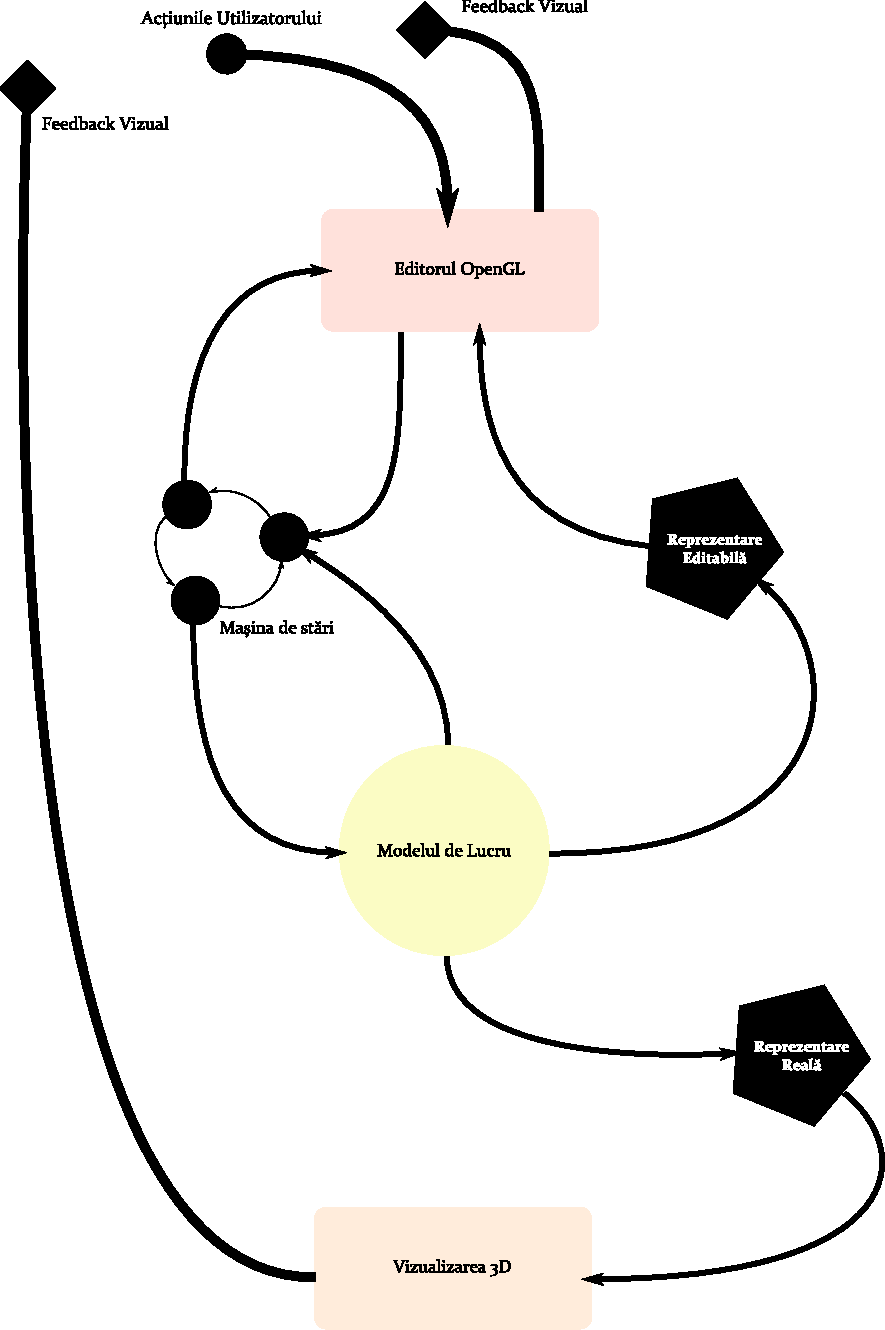
\includegraphics[width=\textwidth]{figures/arh-svg.pdf}
  \caption{Structura generală a proiectului \label{figure:arh}}
\end{center}
\end{figure}

\section{Modelul de lucru}

\begin{definition}
\label{define:model}
Numim \textbf{Model de lucru} reprezentarea într-o colecţie de obiecte Java a 
unei structuri arhitecturale ce poate fi modelată cu ajutorul acestui proiect.
\end{definition}

Modelul de lucru este o reprezentare a unei structuri pe care proiectantul 
doreşte să o reprezinte cu această unealtă într-o formă pe care programul o 
poate recunoaşte şi o poate reface cît mai fidel cu modelul real imaginat de 
proiectant.

\begin{definition}
\label{define:primitive}
Numim \textbf{Primitivă} unitatea structurală şi funcţională a Modelului de 
lucru. O primitivă poate fi o colecţie de alte primitive. De asemenea, o 
primitivă este un element ce poate fi materializat atît la nivel logic cît şi 
într-o reprezentare grafică.
\end{definition}

Primitivele sunt analogiile entităţilor logice în care un model real poate fi 
divizat pentru a-l reprezenta structurat. În seria de primitive ce pot apare în 
modelul logic pot exista primitive care nu au un analog imediat în lumea reală.

\begin{statement}
Modelul logic în totalitatea lui este o Primitivă.
\end{statement}

Plecînd de la aceste două noţiuni, vom încerca să prezentăm întreaga structură 
a Modelului de lucru şi modul în care acesta interacţionează cu aplicaţia în 
sine.

În esenţă, o primitivă este orice poate fi desenat. De aceea, la rîndul său 
modelul este o primitivă. Introducem două direcţii în care modelul poate fi 
reprezentat.

\begin{definition}
\label{define:realRender}
Numim \textbf{Reprezentare Reală} o materializare strictă în comenzi 
Java/OpenGL a unei reprezentări schematice tridimensionale a unei Primitive, 
realizată cu scopul formării unei imaginii asupra rezultatului final al 
construcţiei fizice a entităţii logice din spatele acelei primitive. 
\end{definition} Modelul tridimensional este deci cea mai apropiată formă de 
realitate pe care acest proiect o va reda pentru utilizatorii săi.

\begin{definition}
\label{define:editorRender}
Numim \textbf{Reprezentare Editabilă} o materializare strictă în comenzi 
Java/OpenGL a unei reprezentări schematice bidimensionale a unei Primitive, 
realizată cu scopul identificării vizuale a primitivelor şi accesării facilă 
prin intermediul unui editor a proprietăţilor primitivelor.
\end{definition}

Reprezentarea Editabilă este apropiată ca raţiune figurilor din desenul tehnic, 
şi de aceea identitatea lor vizuală este la rîndul ei asemănătoare acelor 
figuri. Alegerea acestor noţiuni este în strictă corelaţie cu detaliile de 
implementare ale aplicaţiei, care le vom detalia în următorul capitol. Pentru a 
ne face o idee despre cum aceste două reprezentări se potrivesc peste model, 
vom spune că reprezentarea modelului de lucru este juxtapunerea tuturor 
reprezentărilor celorlalte primitive existente în model, în ambele 
reprezentări. Desigur, asta implică că modelul în sine nu este decît un simplu 
container logic pentru toate celelalte componente ale aplicaţiei.

\subsection{Tipuri de primitive}
\label{section:primitives}
Alegerea setului de primitive de care va dispune această aplicaţie a fost o 
sarcină dificilă. Timpul de implementare este în directă corelaţie cu volumul 
de primitive care trebuiesc implementate.

Vom lăsa ca un exerciţiu viitor adăugarea de noi primitive care ar fi de un 
real ajutor utilizatorului acestei aplicaţii. Setul ales este considerat de 
autor ca fiind suficient pentru a oferi un set de funcţionalităţi de bază 
utilizabile pentru această aplicaţie şi destul de variate pentru a scoate în 
evidenţă potenţialul de creştere al acestui proiect.

\subsubsection{Ziduri şi Colţuri de Ziduri}

Elementele constructive esenţiale ale unei structuri sunt zidurile. Ele 
delimitează forma şi suprafaţa construcţiei, avînd un impact crucial asupra 
preţului de construcţie şi facilităţile ce vor putea fi oferite de acea 
construcţie.

Colţurile sunt un tip de primitivă indirect disponibilă proiectantului. Unirea 
capetelor a două ziduri se poate face printr-un colţ, care introduce de fapt o 
legătură permanentă între marginile acelor două ziduri. Constrîngerea este una 
punctuală, zidurile putînd avea orice orientare în cadrul modelului atîta timp 
cît sunt conectate la un colţ. Colţurile pot fi privite ca nişte puncte într-un 
plan.

Orice zid este conectat la două colţuri, \textbf{Colţul de Start} şi 
\textbf{Colţul de Stop}. Astfel poziţionat, lungimea şi orientarea unui zid 
este dictată de poziţia celor două colţuri. Astfel, un zid poate fi privit ca 
un segment ce leagă oricare două puncte (colţuri) dintr-un plan.

\subsubsection{Caracteristici de Ziduri}

\begin{definition}
\label{define:feature}
Numim \textbf{Caracteristică a unui Zid} orice Primitivă ce este asociată în 
mod direct cu un zid.
\end{definition}

Toate Caractersticile sunt constrînse poziţional în lungimea zidului. Ele 
adaugă elemente suplimentare modelului care sunt strict legate în realitate de 
existenţa unui zid. Exemple tipice de caracterstici ce elucidează şi mai bine 
ce reprezintă o caracteristică ar fi:

\begin{itemize}
  \item Fereastră
  \item Uşă
  \item Deschidere -- orice trecere completă prin volumul unui zid (o intrare 
  fără uşă, sau deschiderea unei ferestre fără o fereastră montată în ea)
  \item Cavitate -- orice intrare parţială în volumul unui zid, ca un raft 
  interior într-un perete fals.
  \item Ingroşăre -- orice adăugare la volumul unui zid, o îngroşare într-o 
  anumită zonă, ce poate servi, prin analogie, ca un raft exterior într-un 
  perete.
\end{itemize}
  
\subsubsection{Decoraţiuni}
  
\begin{definition}
\label{define:decoration}
\textbf{Decoraţiunile} sunt Primitive care nu au legătură strictă cu structura 
construită, însă oferă un plus de realism şi poate sugera viitoarea destinaţie 
a diferitelor spaţii din model.
\end{definition}
  
\begin{itemize}
  \item Canapea
  \item Masă
  \item Toaletă
  \item Chiuvetă de baie
  \item Vană
  \item Chiuvetă de bucătărie
  \item Aragaz
  \item Frigider
  \item Masă de bucătărie
\end{itemize}

Dintre aceste Decoraţiuni, unele dintre ele vor fi implementate ca şi 
Caracterstici, datorită constrîngerii lor reale de a apărea pe un zid. Dintre 
cele menţionate mai sus, dăm exemplu chiuveta care întotdeauna apare în 
vecinătatea unui perete.

În Figura \ref{figure:model-arh} vom sumariza cele prezentate mai sus printr-o 
diagramă cu toate componentele modelului de lucru.

\begin{figure}[htp]
\begin{center} 
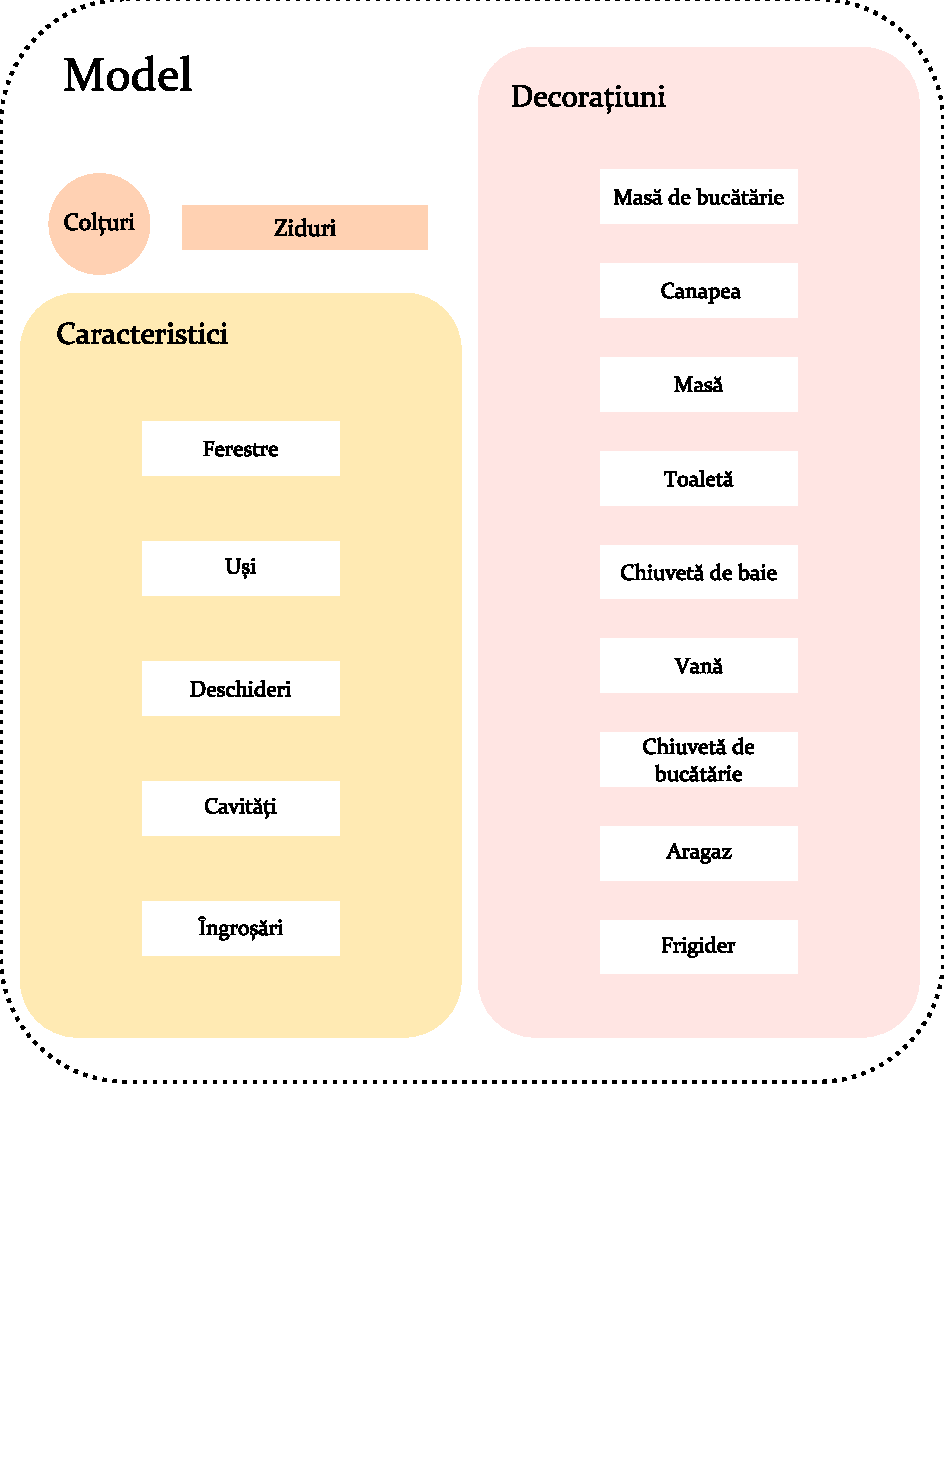
\includegraphics[width=\textwidth]{figures/drawing.pdf} \caption{Arhitectura 
Modelului de Lucru}
  \label{figure:model-arh}
\end{center}
\end{figure}


\section{Editorul OpenGL}
\label{section:opengl-editor}

Înainte de a fi un editor pentru Modelul de Lucru (\ref{define:model}), 
editorul OpenGL dezvoltat de noi este un punct de plecare foarte bun pentru 
orice editor care necesită folosirea facilităţilor OpenGL. Vom încerca să 
descriem succint arhitectura editorului, evidenţiind caracteristicile generice 
cît şi particularizările de suprafaţă care au fost necesare pentru integrarea 
cu funcţionarea dorită.

Editorul este în principiu o suprafaţă de desenare OpenGL cu aspect 
bidimensional ce poate interacţiona cu utilizatorul prin intermediul interfeţei 
oferite de RCP, adică evenimentele ale mausului, ale tastaturii, ale 
vizualizărilor de structură şi de proprietăţi, despre care vom aminti mai jos.

\subsection{Aspecte ale modelului}

\begin{definition}
\label{define:model-aspect}
Numim \textbf{Aspect al Modelului de Lucru} orice formă de interpretare a unei 
primitive aflate într-un model de lucru care nu are legătură cu modelul şi 
structura sa, dar ajută alte componente ale aplicaţiei în a interacţiona cu 
acesta.
\end{definition}

Pentru modelarea funcţionalităţii editorului, orice Primitivă 
(\ref{define:primitive}) este considerată ca un element ce poate fi desenat 
într-un editor. Fiecare Primitivă trebuie să specifice modul în care ea urmează 
să fie desenată în spaţiul bidimensional al editorului.

Unele primitive sunt desenate direct de către model, altele, cum ar fi 
Caracteristicile (\ref{define:feature}), ale căror desenare intră în 
sarcina zidului din care fac parte.

Acest aspect al modelului reprezintă materializarea \textbf{Reprezentării 
Editabile} (\ref{define:editorRender}).

Un alt aspect adăugat modelului este \textbf{Selectabilitate}.

\begin{definition}
\label{define:selectable}
Orice Primitivă care din punct de vedere al interfeţei editorului poate fi 
selectat prin diverse metode de utilizator se spune că este 
\textbf{selectabilă}, sau că are un aspect de \textbf{Selectabilitate}.
\end{definition}

Primitivele pot reacţiona la schimbarea stării lor de selectabilitate şi la 
rîndul său editorul poate trata evenimentul schimbării selecţiei în funcţie de 
implementarea dorită.

În fine, ultimul aspect al modelului necesar implementării editorului este cel 
de \textbf{Navigabilitate}.

\begin{definition}
\label{define:hoverable}
În momentul în care mausul trece deasupra unei 
astfel de componente, ea poate reacţiona prin evenimente implementate la 
nivelul editorului, avînd astfel aspectul de \textbf{Navigabilitate}.
\end{definition}

Multe Primitive folosesc această proprietate pentru a-şi schimba starea de 
selectare.

\subsection{Editorul ca maşină de stări}

Editorul OpenGL funcţionează ca o maşină de stări. Editorul suportă 
înregistrarea stărilor noi şi controlează viaţa tuturor stărilor înregistrate 
în stiva sa de stări.

La un moment dat o singură stare este activă. O stare activă poate controla 
toate evenimentele pe care le primeşte editorul şi poate să introducă noi stări 
în stivă sau să modifice modelul în funcţie de evenimentele care au avut loc. 
Starea decide cînd viaţa ei a luat sfîrşit. Această decizie este comunicată 
editorului care apoi deînregistrează starea din stivă.

În Tabela \ref{table:editor-states} vom prezenta ciclul de viaţă al unei stări. 
Acest model de ciclu de viaţă a fost stabilit în funcţie de necesităţile 
editorului OpenGL, pentru a-i permite acestuia să interacţioneze sincron cu 
schimbările de stare ce pot fi controlate asincron de către evenimentele 
aplicaţiei.

Dintr-o anumită privinţă, acest ciclu de stare poate fi privit ca o serie de 
meta-stări ale aplicaţiei (i.e. stări ale stărilor).

\begin{table}[ht] \caption{Ciclul de viaţă al stărilor Editorului OpenGL
\label{table:editor-states}}
\begin{tabular}{|\col{0.23}|\col{0.73}|}

\hline FRESH & La construcţia unei stări ciclul de viaţă este setat în poziţia 
FRESH. Editorul va citi orice stare setată pe acest mod şi o va seta ca şi 
stare activă, înregistrînd toate rutinele de tratare a evenimentelor pentru 
această stare în cadrul editorului. Starea curentă este setată ca activă şi 
modul ei este trecut în RUNNING. Starea activă anterioară este trecută pe modul 
SLEEPING. \\

\hline RUNNING & După ce editorul iniţializează o stare, ea este în modul 
RUNNING. În acest mod starea primeşte toate evenimentele editorului. Decizia de 
a părăsi această stare se poate lua după două criterii. a) La discreţia stării 
în sine, prin trecerea în modul TERMINATED sau b) la discreţia editorului, în 
momentul sosirii unei noi stări FRESH, cînd starea curentă trece în SLEEPING. \\

\hline SLEEPING & Toate stările care au fost oprite de editor la apariţia unei 
stări noi se adună într-o stivă şi modul lor este trecut în SLEEPING. Ele pot 
sta în acest mod un timp nedefinit şi pot să nu-l părăsească niciodată. Ele pot 
reveni la starea RUNNING în momentul în care se află la vîrful stivei şi starea 
activă trece în modul TERMINATED. Atunci editorul automat va muta starea din 
capul stivei ca stare activă şi ea va deveni RUNNING. De aceea rutina de 
tratare a tranziţiei în RUNNING cît şi rutina de tratare în starea TERMINATED 
trebuie să aibă în vedere posibilitatea rulării de mai multe ori pentru aceeaşi 
stare (i.e. să nu trateze iniţializări, care se fac în mod normal în starea 
FRESH) \\

\hline TERMINATED & Odată ce starea consideră că şi-a încheiat activitatea, ea 
poate alege să treacă în modul TERMINATED. Odată ajunsă în acest mod, starea va 
fi deînregistrată din lista de captare a evenimentelor editorului şi va fi 
scoasă permanent din lista stărilor editorului.\\

\hline
\end{tabular}
\end{table}

Stările editorului sunt folosite pentru a manipula modelul de lucru. Ele pot 
adăuga şterge sau schimba diverse proprietăţi ale primitivelor aflate în model. 
Din acest motiv, stările sunt strict asociate cu diversele tipuri de primitive 
din model.

De exemplu, colţurile introduc o serie de stări pentru a le modela toate 
operaţiunile posibile în cadrul editorului. Ele pot fi enumerate după cum am 
arătat în Tabela \cite{table:corner-states}.

\begin{table}[ht] \caption{Stările ce modelează operaţiile posibile pentru 
diverse Primitive \label{table:corner-states}}
\begin{tabular}{|\col{0.23}|\col{0.73}|}
\hline \multicolumn{2}{|l|}{\Large \textbf{Colţuri}} \\
\hline DragCornerState & Modelează modificarea poziţiei unui colţ atunci cînd 
el este tras cu mausul pe suprafaţa editorului. \\
\hline SelectCornerState & Implementează comportamentul operaţiunii de 
selectare a unui Colţ. Dacă selecţia s-a făcut fără ca mausul să fie în 
vecinătatea colţului, atunci starea se termină imediat, altfel se iniţiază 
DragCornerState. \\ \hline \multicolumn{2}{|l|}{\Large \textbf{Ziduri}} \\
\hline PickupCornerState & Modelează operaţiunea de alegere a unui colţ în
cadrul sarcinii de adăugare a unui zid.

\\ \hline
\end{tabular}
\end{table}

% TODO Adaugă toate stările posibile în descriere

\subsection{Capacităţi asincrone}

Editorul OpenGL este optimizat pentru motorul asincron de sincronizare, 
desenare şi tratare a evenimentelor ale aplicaţiilor Eclipse RCP. Deşi vom 
intra în detalii în capitolul \ref{chapter:impl}, amintim doar aici că într-o 
singură aplicaţie se pot edita oricîte Modele de Lucru, fără nici un impact 
asupra unuia dintre ele şi fără interferenţe de nici un fel atît în logica 
modelului cît şi în ciclul de randare.

\section{Vizualizarea 3D OpenGL}
\label{section:view}

După cum am văzut în secţiunea \ref{section:opengl-editor}, Editorul OpenGL 
serveşte la manipularea Modelului de Lucru (\ref{define:model}) şi a 
proprietăţilor diverselor Primitive (\ref{define:primitive}) din acest Model. 
Sarcina vizualizării tridimensionale a modelului cade în măinile componentei 
despre care vom discuta în această secţiune.

Diferenţa principală dintre Editor şi Vizualizare este că cea din urmă nu 
permite interacţiunea cu proprietăţile modelului, ci doar proiecţia lor într-o 
lume tridimensională. Proiecţia se face într-o scenă văzută în perspectivă şi 
cu toate obiectele desenate prin contur cu muchiile din spate ascunse. Modelul 
poate fi explorat cu ajutorul mausului, însă nu se poate interacţiona în nici 
un fel similar cu capacităţile editorului.

\subsection{Aspectul de desenare reală}

La rîndul său, Vizualizarea 3D introduce un aspect (\ref{define:model-aspect}) 
asupra Modelului de Lucru. Acest aspect este cel de \textbf{desenare reală}. 
Deşi structura ierhahică a liniei de randare este similară cu cea a aspectului 
de randare pentru editare, există o singură diferenţă semnificativă.

Pentru randarea scenei cu contur ascunzînd muchiile din spate, OpenGL necesită 
ca scena să fie randată în două treceri. Prima trecere reprezintă volumele de 
randare şi în a doua trecere se desenează contururile.

În principiu, aspectul de desenare reală trebuie să aibă în vedere optimizarea 
celor două treceri pentru a obţine doar acele contururi care sunt de interes 
pentru utilizator, fără a marca toate poligoanele din scenă.

\subsection{Conexiunea cu Editorul OpenGL}

Precum Editorul OpenGL, Vizualizarea 3D OpenGL are şi ea ample capacităţi 
asincrone, răspunzînd la solicitările editorului şi putînd servi simultan 
nevoile a mai multor editoare. Platforma RCP forţează ca orice vizualizare să 
existe o singură dată în interfaţa grafică. Prin această limitare se impune ca 
Vizualizarea 3D să reprezinte doar modelul aflat în Editorul activ la un moment 
dat.

De asemenea, Vizualizarea 3D are capacitatea de a reprezenta orice modificare
are loc în Modelul de Lucru în timp real, în momentul în care datele parţiale
sunt salvate în Model.

	\chapter{Implementare}
\label{chapter:impl}

În acest capitol vom prezenta detaliile implementării acestui proiect. Se va 
trece prin structura de clase, fluxul datelor în aplicaţie, mutaţiile Modelului 
de Lucru (\ref{define:model})  şi funcţionarea componentelor de interfaţă, 
editorul OpenGL şi Vizualizarea 3D, prezentate în secţiunile 
\ref{section:opengl-editor}, respectiv \ref{section:view}.

Vom trece în revistă, de asemenea, principalele conexiuni la nivel de cod între 
componentele aplicaţiei, şi modul de interacţiune al principalelor module 
prezentate în Capitolul \ref{chapter:arh}.

Fiecare dintre componentele arhitecturale descrise la capitolul 
\ref{chapter:arh} sunt materializate în implementarea efectivă printr-un set de 
clase bine definite şi bine separate ca logică şi structură de celelalte 
componente ale aplicaţiei.

Există o diviziune clară între componentele abstracte, definitorii ale 
aplicaţiei noastre şi componentele materializate, implementările concrete. 
Toate abstracţiile făcute aici reprezintă forme de simplificare a 
interacţiunilor între obiecte, de marcare a anumitor comportamente şi separarea 
sarcinilor de dezvoltare în unităţi logice ce pot fi urmărite pe direcţia mai 
multor module de cod ale programului.

\section{Modelul de Lucru}

\subsection{Model}
Există o clasă specială pentru concretizarea conceptului de Model 
(\ref{define:model}). Responsabilităţile modelului cad în a fi un suport logic 
cît şi structural pentru obiectele ce materializează componentele modelului 
proiectat de către utilizator. Pentru asta, clasa model va şti întotdeauna 
diverse informaţii vitale funcţionării editorului.

Modelul în sine implementează aspectele de desenare pentru proiectate 
(\ref{define:editorRender}) şi de desenare reală (\ref{define:realRender}). 
Reutilizarea abstracţiei despre care vom vorbi imediat la Primitive conferă 
coerenţă şi creşte şi mai mult nivelul de abstactizare la care se poate lucra 
cu această aplicaţie.

Îndeplinirea sarcinilor de editare pentru proiectare şi de desenare reală se 
rezumă la apelarea aceloraşi rutine pentru toate componentele modelului. Pentru 
a reţine toate componentele, clasa de faţă reţine tabele de căutare pentru 
toate componentele care aleg să fie înregistrate în model.

Pot exista primitive care nu sunt desenate direct de către model, în speţă este 
cazul Caracteristicilor (\ref{define:feature}). Acestea sunt desenate de 
containerul lor, în speţă Zidul care le conţine.

Modelul serveşte şi ca suport pentru persistenţa datelor. Salvarea datelor în 
formatul specific aplicaţiei de faţă reprezintă varianta serializată a clasei 
model. De aceea, este important ca toate datele care sunt necesare salvării 
stării modelului să fie prezente cumva în legătură cu modelul, altfel există 
şansa ca ele să nu fie persistate de către aplicaţie în momentul în care se 
salvează în fişier documentul de lucru.

Modelul serveşte şi ca suport sumar de reţinere de stare pentru Editorul 
OpenGL. El va păstra în model selecţia curentă, cît şi starea transientă a 
unora dintre componente, cum ar fi dacă ele sunt navigate de către maus la 
momentul respectiv sau nu.

Aceasta se realizează prin păstrarea informaţiei despre elementele ce pot fi 
navigate (i.e. care implementează aspectul de Navigabilitate 
(\ref{define:hoverable})) într-o tabelă de căutare specială. Editorul va cere 
reevaluarea deciziei de navigabiltiate pentru toate componentele din această 
listă în momentul în care mausul îşi modifică poziţia în urma acţiunii 
utilizatorului.

\subsection{Primitive}
Clasa de bază a modelului de lucru este clasa Primitive. Desigur, este o 
materializare a conceptului de Primitivă (\ref{define:primitive}). Aceasta este 
o clasă abstractă care nu introduce nici un comportament singular, însă 
marchează nevoie de implementare pentru intefeţele EditorRenderable şi 
RealRenderable, necesare celor două vizualizări, cum vom vedea la secţiunile 
\ref{section:impl-editor} şi \ref{section:impl-view}.

Din clasa Primitive sunt extinse clasele concrete Corner, Wall şi toate clasele 
ce implementează Decoraţiunile (\ref{define:decoration}). Fiecare din aceste 
clase implementează metodele definite în interfeţele amintite mai sus.

Tot din clasa Primitive se desprinde şi clasa WallFeature, o materializare a 
conceptului de Caracterstică de Ziduri (\ref{define:feature}). Din ea la rîndul 
ei se concretizează clasele Door, Window, Inset, Outset, Tunnel, implementări 
ale diverselor caracteristici amintite în \ref{section:primitives}.

Deşi este doar o clasă de marcaj, Primitive prezintă un rol crucial în cadrul 
arhitecturii aplicaţiei noastre. Întreaga interacţiune pe care o au editorul şi 
vizualizarea 3D cu modelul se face prin această abstracţie. Tot ce are nevoie 
să ştie modelul despre orice componentă a sa este că extinde clasa Primitive. 
Cu această minimă funcţionalitate, se pot implementa toate operaţiile de 
desenare necesare interfeţei aplicaţiei de faţă.

\subsection{Corner}

Clasa Corner reprezintă una din puţinele Primitive care nu sunt direct 
disponibile utilizatorului aplicaţiei. Ea serveşte strict poziţionării 
Zidurilor şi prin aceasta editorul nu le oferă o importanţă deosebită printr-o 
individualizare în cadrul interfeţei, reducînd astfel solicitarea asupra curbei 
de învăţare a utilizatorului.

Clasa Corner, pe lîngă implementarea comportamentului de desenare pentru 
proiectate (\ref{define:editorRender}) şi de desenare reală 
(\ref{define:realRender}), aderă şi la comportamentele de Selectabilitate 
(\ref{define:selectable}) şi de Navigabilitate (\ref{define:hoverable}).

Ironic este însă că deşi joacă un rol atît de important în poziţionarea 
obiectelor în scenă, şi interacţionează mai mult decît orice altă componentă cu 
utilizatorul, colţurile nu au reprezentare specifică în editor. Deşi există un 
marcaj pentru starea de selecţie a colţului, în rest imaginea colţului este de 
fapt inexistentă. Îmbinarea lor cu alte componente şi efectul care îl au asupra
 Zidurilor îi oferă o reprezentare sugestivă şi pot fi controlate astfel de 
către utilizator.

\subsection{Wall}

Materializarea zidurilor are un rol important în cadrul aplicaţiei pentru că 
serveşte la rîndul său ca un container pentru toate tipurile de Caracteristici 
(\ref{define:feature}) ce pot fi adăugate în model. În acest scop, clasa reţine 
o listă sortată cu toate caracteristicile ce există pe acel Zid.

\begin{figure}[htp]
\begin{center}
  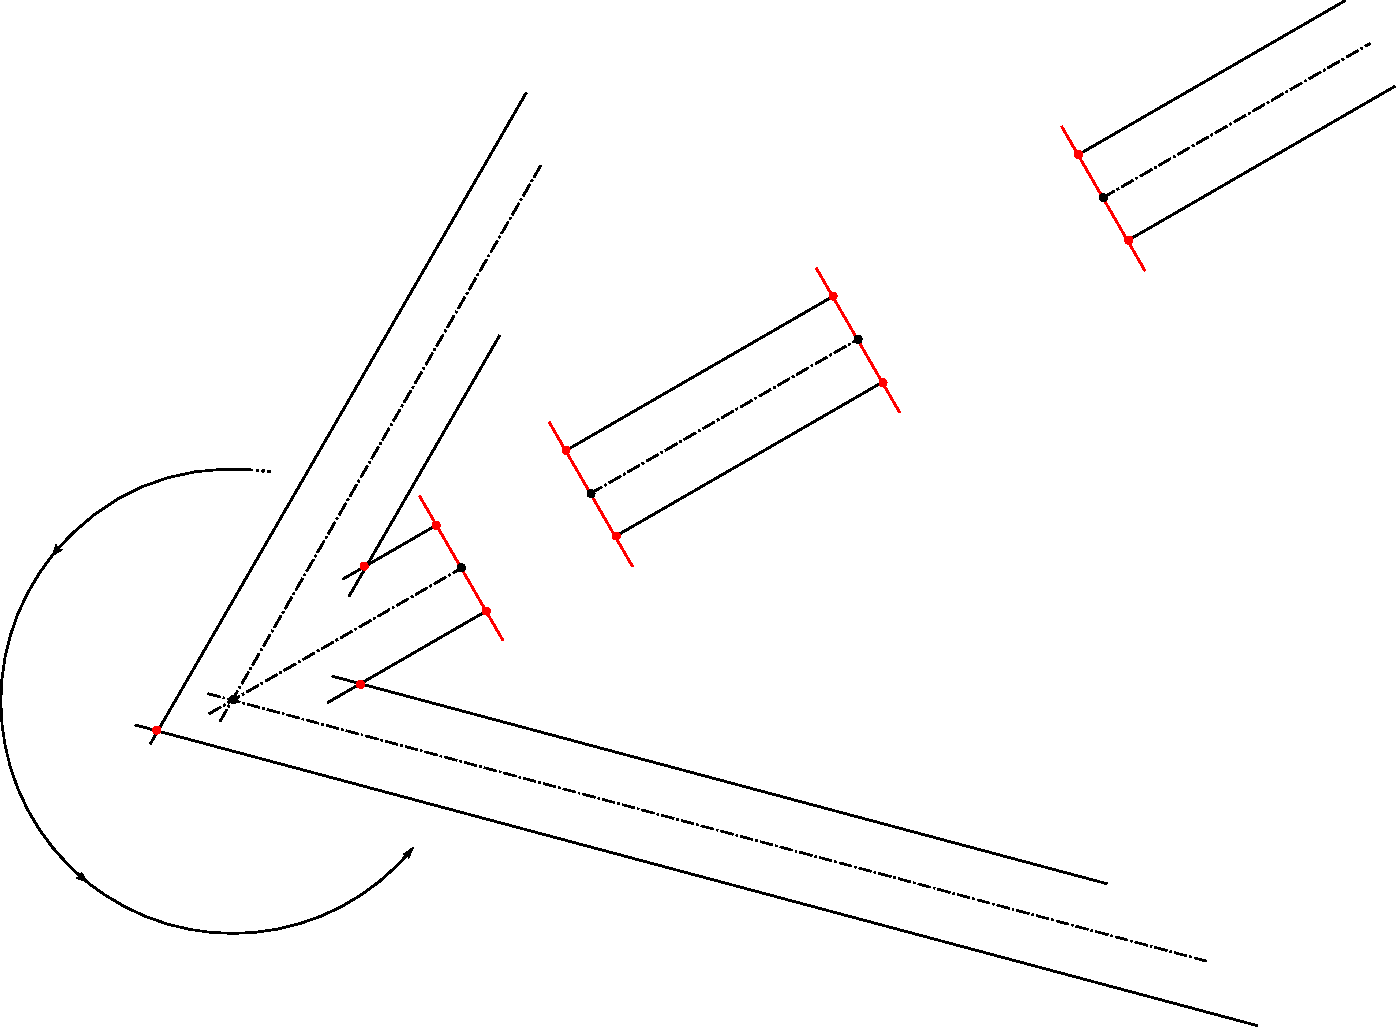
\includegraphics[width=0.9\textwidth]{figures/corners.pdf}
  \caption{Determinarea liniilor de contur pentru un Zid \label{figure:corner}}
\end{center}
\end{figure}

Destul de interesantă este metoda de desenare a zidurilor care, atît pentru 
desenarea reală cît şi pentru cea destinată editorului, aplică un algoritm de 
unire cu ceilalţi pereţi ce împart acelaşi colţ. Algoritmul calculează, 
printr-o parcurgere în sens trigonometric a tuturor zidurilor conectate la un 
colţ, interesecţia dintre muchiile interioare şi exterioare cu pereţii 
alăturaţi, aşa cum se poate vedea în Figura \ref{figure:corner}. Apoi se 
trasează liniile exterioare şi interioare pînă în punctele respective. Există, 
desigur, cazuri limită în care liniile trebuie eliminate datorită faptului că 
intersecţia depăşeşete dimensiunea reală a zidului şi atunci linia ar fi 
desenată de fapt în afara conturului zidului respectiv.

Zidurile sunt responsabile şi de desenarea tuturor Caracteristicilor aflate pe 
zid. Pentru aceasta, conturul exterior al zidurilor trebuie întrerupt în locul
în care caracteristica urmează să fie desenată. Această decupare este îmbinată
cu algorimtul de detectare a intersecţiilor cu celelalte ziduri din colţ. pentru
fie care dintre laturile zidurilor, se calculează punctele de intersecţie dintre
punctele ce delimitează fiecare caracteristică şi muchiile zidurilor, cum am
arătat în Figura \ref{figure:corner}.

Apoi, în spaţiul vid creat de delimitările tuturor caracteristicilor, printr-o
transformare afină, se mută sistemul de coordonate rotit şi poziţionat în
punctul de start al fiecărei caracterstici. În final se apelează rutina de
desenare a caractersticii, fie cea reală sau cea pentru editare, după caz.

\subsection{WallFeature}

Feature este clasa care marchează toate caracteristicile ce pot apărea pe un
Zid. Nu vom repeta enumerarea lor de la Secţiunea \ref{section:features}, ci vom
încerca să prezentăm modalitatea în care am implementat funcţionalitatea
acestora.

Practic, pentru fiecare caracteristică, cum am arătat la secţiunea precedentă,
zidul este prevăzut cu o cavitate în care desenarea este lăsată pe baza
caracteristicii. Dacă caracteristica nu ocupă întregul volum al zidului în zona
respectivă, este responabilitatea ei să ``cîrpească'' înapoi zidul, cum este
cazul ferestrelor, care lasă intact peretele în partea inferioară şi superioară
ferestrei în sine, sau la fel pentru uşi care au un spaţiu pînă la tavan.

Fiecare caracteristică trebuie să ofere propria reprezentare grafică, însă ele
sunt scutite de nevoile calculaţiilor poziţionale\footnote{Precum nu sunt
scutite zidurile, al căror algoritm de determinare a muchiilor implică calcule
complexe}, datorită faptului că zidurile aplică o transformare afină înainte de
iniţierea procedurii de desenare a caracteristicii, mutînd spaţiul de coordonate
în punctul de start al caractersticii şi cu rotaţia corespunzătoare.

\subsection{Decoration}

Decoraţiunile sunt componente independente de celelalte elemente de model, ce
sunt desenate poziţional direct de către model (precum zidurile). Simplitatea
lor implică puţine dificultăţi tehnice. Fiecare dintre ele a trebuit însă
proiectată cu grijă pentru a reda modelul reprezentat cît mai aproape posibil de
imaginea reală.

Cum este valabil şi pentru ziduri, nu se face detectare a suprapunerilor peste
alte obiecte, fiind astfel posibil ca diverse decoraţiuni să se suprapună peste
altele sau peste ziduri. O implementare rudimentară ar putea evita cele mai
multe din situaţiile de suprapunere, folosind funcţiile de suprapunere
implementate de fiecare obiect în parte.

\section{Editorul OpenGL}
\label{section:impl-editor}

\subsection{Integrarea cu Eclipse}
Editorul OpenGL este un editor pentru Eclipse RCP, şi respectă standardele
pentru un editor de acest fel. De aceea, el poate fi folosit ca orice alt editor
(i.e. Un editor de text pentru surse Java) în cadrul unei aplicaţii Eclipse. El
este integrat cu Eclipse şi se marchează ca editor standard pentru fişiere de
tip .ocm\footnote{Extensia standard a fişierelor acestui proiect: OpenCad.org
Model}.

Desigur, diferenţa majoră faţă de alte editoare întîlnite în Eclipse este că
prezentarea sa nu se face prin intermediul unui control de editare de text, ci
printr-o suprafaţă de desenare OpenGL. Cea mai mare parte a pragurilor care au
trebuit trecute în implementarea acestei aplicaţii au derivat din această
caracteristică deosebită a editorului nostru.

Editorul are o sursă de selecţie şi paginator de conţinut, a căror descriere o
vom prezenta în \ref{section:impl-selecta}. Prin această componentă, spunem că
Editorul OpenGL este integrat perfect cu Eclipse RCP, beneficiind (poate
beneficia astfel) de toate facilităţile pe care le are de oferit această
platformă.

\subsection{Plugin-ul OpenGL pentru SWT}
Editorul OpenGL este primul loc al aplicaţiei unde avem de aface cu plugin-ul
pentru OpenGL şi SWT. Deşi a fost scris special pentru Eclipse, acest plugin a
necesitat o extensivă testare şi configurare pentru funcţionarea corectă alături
de platforma Eclipse.

Plugin-ul de OpenGL funcţionează pe baza unei suprafeţe de desenare\footnote{O 
clasă numită GLCanvas}. În cadrul unei aplicaţii pot exista mai multe astfel de 
suprafeţe, \footnote{În cazul nostru era strict necesar existenţa a mai mult de 
o astfel de suprafaţă, datorită posibilităţii de a avea mai multe editoare, şi 
posibilitatea de a avea simultan Vizualizarea 3D} dar în orice moment o 
instrucţiune OpenGL nu poate desena decît într-o singură anume astfel de 
suprafaţă, desemnată printr-o rutină de selectare. Prima implementare (cea 
directă) a avut ca rezultat ``scurgerea'' de diverse efecte şi secţiuni din 
desen dintr-o suprafaţă în alta, datorită problemelor de sincronizare datorate 
de faptul că Eclipse RCP execută diverse operaţiuni în fire de execuţie 
diferite, care executau simultan instrucţiuni OpenGL fără o determinare precisă 
a suprafeţei în care ele desenau. Soluţia a fost sincronizarea diverselor 
metode din Editor şi Vizualizarea faţă de un punct fix, şi în cadrul zonei 
sincronizate să se selecteze (şi astfel să fie totdeauna determinată) suprafaţa 
de desenare.

\subsection{Maşina de stări}
Pentru implementarea maşinii de stări am folosit o stivă în vîrful căreia stătea
totdeauna starea activă\footnote{Am explicat funcţionarea Maşinii de stări în
Secţiunea \ref{section:machine}}.

Întreg comportamentul editorului este modelat prin intermediul acestor stări.
Pentru preluarea şi retragerea controlului anumitor stări asupra suprafeţei de
editare, se folosesc metode de aflare a unor obiecte de tratare a evenimentelor
pentru diverse evenimente ale editorului. Tipurile de obiecte de tratare sunt
prezentate în Tabela \ref{table:state-events}.

\begin{table}
\begin{tabular}{{|\col{0.28}|\col{0.68}|}}
\hline
\textbf{Clasă} & \textbf{Descriere Funcţionare}
\\ \hline
KeyListener & Poate interpreta orice apăsare de tastă (sau respectiv eliberare
de tastă, prin intermediul unui cod care indentifică unic orice tastă)

\\ \hline
MouseListener & Interceptează apăsările butoanelor mausului, fie cu click simplu
sau dublu, fiind capabil să reacţioneze la toate aceste evenimente, avînd
cunoştinţe asupra zonei în care mausul a fost apăsat.

\\ \hline
MouseMoveListener & Tratează orice mişcare a mausului în suprafaţa editorului şi
poate executa o rutină incrementală la fiecare deplasare a mausului.

\\ \hline
MouseTrackListener & Poate intercepta evenimentele de intrare a mausului, de
ieşire a acestuia şi starea de deplasare deasupra suprafeţei editorului.

\\ \hline
MouseWheelListener & Interceptează orice mişcare a rotiţei mausului pentru a
reacţiona în funcţie de viteza de rotaţie şi poziţia mausului în acel moment. De
notat că acest tip de eveniment nu are o clasă proprie ci se lucrează direct cu
interfaţa generică Listener.

\\ \hline
\end{tabular}
\caption{Tipurile de evenimente ce pot fi tratate de o stare a editorului
\label{table:state-events}}
\end{table}

\subsection{Interacţiunea cu utilizatorul. Prezentarea 2D}
Editorul OpenGL poate interacţiona prin intermediul mausului cu orice obiect din
model ce suportă acest comportament. Pentru aceasta, editorul trebuie să reţină
în orice moment caracteristicile zonei care este desenată pe ecran, adică
punctul de start, dimensiunile în coordonate model ale ferestrei de afişare. La
fiecare interacţiune cu mausul, coordonatele ecran sunt transformate în
coordonate model cu ajutorul acestor informaţii.

Editorul are, de asemenea, capacitatea de a modifica valorile de vizualizare
într-un mod intuitiv, care-i permite să vizualizeze diverse detalii ale
modelului la diverse scări de mărire. Utilizatorul poate controla aceste
caracteristici cu ajutorul stării de navigare, în care tragerea suprafeţei de
editare mută punctul de start iar scroll-ul cu rotiţa modifică scara desenului.

De asemenea, redimensionarea ferestrei va mări suprafaţa de desenare după un
algoritm special. Pe scurt, acest algoritm încearcă să păstreze aceeaşi mărire
relativă a modelului\footnote{Se păstrează aceeaşi cantitate de detalii în
desen}, la acelaşi aspect al ferestrei de vizualizare. La modificare aspectului,
cantitatea de detalii va ramîne constantă în zona pătratică a desenului,
crescînd înspre zonele unde modificarea aspectului scoate la iveală noi zone din
model.

\section{Vizualizarea 3D}
\label{section:impl-view}

\subsection{Integrarea cu Eclipse}
Vizualizarea 3D este o Vizualizare Eclipse standard. Ca şi în cazul editorului,
particularitatea componentei create de noi este că foloseşte pentru
reprezentarea conţinutului o suprafaţă de desenare OpenGL. Diferenţa
fundamentală faţă de Editor este căm în cazul vizualizării, utilizatorul nu
poate modifica modelul de lucru prin interacţiunea cu controlul respectiv.
Astfel, se reduce mult din nevoile şi calculaţiile necesare (nu avem nevoie nici
de mecanismul de stări prezent la editor). Vizualizarea este doar o modalitate
foarte bună de vizualizarea tridimensională a modelului final.

\subsection{Prezentarea 3D}
Deşi toate rutinele de desenare sunt prezente în fiecare componentă a modelului
în parte, vizualizarea are însă totuşi responsabilitatea de a face unele
operaţii pentru suprafaţa de desenare.

În principal, are aceleaşi responsabilităţi de sincronizare de threaduri pe care
le are şi Editorul. Deşi nu poate exista decît o singură vizualizare, motorul de
desenare OpenGL interacţionează în acelaşi fel cu toate componentele care doresc
să deseneze pe o suprafaţă OpenGL.

De asemenea, vizualizarea are răspunderea de a seta datele proiecţiei, în
funcţie de unghiul de privire şi punctul de centru pe care utilizatorul le poate
modifica cu ajutorul mausului. Pentru controlul acestor coordonate, vizualizarea
captează evenimentele mausului întocmai ca o stare a editorului şi tratează
diverse mişcări ale mausului în sensul modificării parametrilor de vizualizare.

\section{Sursa de selecţie}
\label{section:impl-selecta}
Sursa de selecţie, reprezentată de clasa GLEditorOutlinePage serveşte în 
principal vizualizării de structură, prezentată la \ref{section:impl-outline}. 
Însă în acelaşi timp, serveşte unui scop similar sincronizării cu Vizualirea 
3D. Principala ei funcţie este să anunţe tuturor celor înscrişi schimbarea 
selecţiei în editor. Schimbarea selecţiei poate avea mai multe 
surse\footnote{i.e. Vizualizarea structurii poate schimba selecţia}, şi deci şi 
editorul în sine ascultă acest serviciu. Pentru aceasta, el trebuie să se
protejeze la a reacţiona în lanţ la acţiunea de schimbare a
selecţiei\footnote{El cînd schimbă selecţia anunţă serviciul, care apoi îl
anunţă pe el, el schimbă selecţia şi anunţă din nou, etc.}.

În acelaşi timp clasa menţionată serveşte ca sursă de conţinut pentru
Vizualizarea de structură. Arborii în SWT sunt structuri abstracte, care separă
conţinutul de prezentare, şi partea lor de sursă de date este tocmai această
clasă.

\section{Vizualizarea structurii}
\label{section:impl-outline}

Vizualizarea de structură se bazează în principal pe Sursa de selecţie, descrisă
la \ref{section:impl-selecta}. În general, toate editoarele din Eclipse
beneficiază de această componentă, şi utilizatorul se aşteaptă ca în cadrul ei
să vizualizeze toate componentele logice într-o structura naturală.

În cazul de faţă, se prezintă toate primitivilele şi conexiunile dintre ele,
într-o structură arborescentă. Deşi legăturile dintre primitive sunt mai
complexe, se reprezintă într-o versiune simplificată şi uşor de înţeles pentru
utilizator.

Conţinutul efectiv al vizualizării este dat de sursa de selecţie, prezentată la
\ref{section:impl-selecta}. Vizualizarea de structură este doar o componentă
standard a Eclipse RCP, particularizată prin conectarea cu sursa de selecţie.

\section{Particularizările interfeţei Eclipse}

	\chapter{Concluzii}

Good, Good...
\clearpage
	\pagenumbering{roman}
	\bibliographystyle{acm}
	\bibliography{thesis}
\end{document}